\documentclass[11pt,aspectratio=43,usenames,dvipsnames]{beamer}
\usepackage[utf8]{inputenc}
\usepackage{amsmath, amsfonts, amssymb, amsthm}
\usepackage[T1]{fontenc}
% mint: code chuck and syntax highlighting
%% outputdir should change according to pdf build directory
\usepackage[outputdir=build,cache=false]{minted}
\usepackage{lmodern}
\usepackage{xcolor}
\usepackage{setspace}
\usepackage{booktabs}
\usepackage{multirow}
\usepackage{graphicx}
\usepackage{fontawesome}

\usepackage[mode=tex]{standalone}
\usepackage{tikz}
\usetikzlibrary{decorations}
\usetikzlibrary{decorations.pathreplacing, intersections}
\usepackage{pgfplots}
\usetikzlibrary{calc,positioning}
\usepgfplotslibrary{fillbetween}
\pgfplotsset{compat=newest, scale only axis, width = 10cm}

% ---------------------------------------------------------------------
% Coordinate extraction
% #1: node name
% #2: output macro name: x coordinate
% #3: output macro name: y coordinate
\newcommand{\Getxycoords}[3]{%
    \pgfplotsextra{%
        % using `\pgfplotspointgetcoordinates' stores the (axis)
        % coordinates in `data point' which then can be called by
        % `\pgfkeysvalueof' or `\pgfkeysgetvalue'
        \pgfplotspointgetcoordinates{(#1)}%
        % `\global' (a TeX macro and not a TikZ/PGFPlots one) allows to
        % store the values globally
         \global\pgfkeysgetvalue{/data point/x}{#2}%
         \global\pgfkeysgetvalue{/data point/y}{#3}%
     }%
}
% ---------------------------------------------------------------------

\usepackage{ulem}
\usepackage{hyperref}
\usepackage{booktabs}
\usepackage{babel}
\usepackage{makecell}
\usepackage[para,online,flushleft]{threeparttable}
\usepackage{pdfpages}
\usepackage{tcolorbox}
\usepackage{bm}
\usepackage{appendixnumberbeamer}
\usepackage{natbib}
\usepackage{caption}
\captionsetup[figure]{labelformat=empty}% redefines the caption setup of the figures environment in the beamer class.
\usetheme[compress]{Boadilla}
\usecolortheme{default}
\useoutertheme{miniframes}
\usefonttheme[onlymath]{serif}

\newcommand{\jump}[2]{\hyperlink{#1}{\beamerbutton{#2}}}
\newcommand{\extjump}[2]{\href{#1}{\beamerbutton{#2}}}
\newcommand{\orange}[1]{\textcolor{orange}{#1}}
\newcommand{\red}[1]{\textcolor{red}{#1}}
\newcommand{\blue}[1]{\textcolor{blue}{#1}}
\newcommand{\green}[1]{\textcolor{OliveGreen}{#1}}

\renewcommand{\square}{\scalebox{0.7}{$\blacksquare$ \hspace{0.5em}}}
\setbeamertemplate{itemize item}{\raisebox{0.1em}{\scalebox{0.7}{$\blacksquare$}}}
\setbeamertemplate{itemize subitem}[circle]
\setbeamertemplate{itemize subsubitem}{--}
\setbeamercolor{itemize item}{fg=black}
\setbeamercolor{itemize subitem}{fg=black}
\setbeamercolor{itemize subsubitem}{fg=black}
\setbeamercolor{item projected}{bg=darkgray,fg=white}
\definecolor{blue}{rgb}{0.2, 0.2, 0.7}
\setbeamercolor{alerted text}{fg=blue}
\setbeamertemplate{enumerate items}[circle]


\setbeamertemplate{headline}{}

%==========================================
\let\olditemize=\itemize
\let\endolditemize=\enditemize
\renewenvironment{itemize}{\olditemize \itemsep1em}{\endolditemize}
\let\oldenumerate=\enumerate
\let\endoldenumerate=\endenumerate
\renewenvironment{enumerate}{\oldenumerate \itemsep1em}{ \endoldenumerate}

\DeclareMathOperator*{\argmax}{\arg\!\max}
\DeclareMathOperator*{\E}{\mathbb{E}}
\DeclareMathOperator*{\var}{\rm Var}
\DeclareMathOperator*{\cov}{\rm Cov}

\theoremstyle{definition}
\newtheorem{assume}{Assumption}
\newtheorem{lem}{Lemma}
\newtheorem{proposition}{Proposition}
\newtheorem{thm}{Theorem}
\newtheorem{corol}{Corollary}

\AtBeginSection[]{
  \begin{frame}[noframenumbering]
  \vfill
  \centering
  \begin{beamercolorbox}[sep=8pt,center,shadow=true,rounded=true]{title}
    \usebeamerfont{title}\insertsection\par%
  \end{beamercolorbox}
  \vfill
  \end{frame}
}

\begin{document}
    \title[Unit 13]{Unit 13 \\ Economics Fluctuations and Unemployment }
    \author[Hui-Jun Chen]{Hui-Jun Chen}
    \institute[OSU]{The Ohio State University}
    % \date{\today}
    \date{\today}
    \setbeamertemplate{navigation symbols}{}
    \setstretch{1.2}

%-------------------------------------------------------
{
%	\usebackgroundtemplate{\includegraphics[width=1\paperwidth]{../EveningSky_cropped_edit43_bright.jpg}}
    \begin{frame}
% \vspace{3em}
        \centering
%		{\footnotesize 	ECON 4002 Intermediate Macroeconomic Theory}
        \maketitle
% \vspace{-1.5em}
% \centering
% \includegraphics[width=0.55\linewidth]{Pictures/houses.jpeg}


    \end{frame}
}

% -------------------------------------------
\setbeamertemplate{headline}
{
\setbeamercolor{section in head/foot}{fg=black, bg=white}
\vskip1em \tiny \insertsectionnavigationhorizontal{1\paperwidth}{\hspace{0.50\paperwidth}}{}
}
%------------------------------------------

\section[Intro]{Introduction}
\label{sec:Introduction}

\begin{frame}{Introduction \extjump{https://www.core-econ.org/the-economy/book/text/13.html}{Textbook}}
\label{slide:Introduction}

\begin{itemize}
    \item In Unit 10, we introduced \textit{time} to individual
    \begin{itemize}
        \item intertemporal substitution, bank \& financial system \ldots
    \end{itemize}
    \item Recall Lucas' critique: \alert{agg. behavior replies on micro foundation}
    \item What are the \textbf{dynamics} of the whole economy? (business cycle)
    \item How to measure aggregate economy? ($3$ approach on GDP)
    \item What drives the agg. dynamics? (Econ Fluctuations \& Investment)
    \item Does price have dynamics? (Inflation)
\end{itemize}
\end{frame}

\section[\faRefresh]{The Business Cycle}
\label{sec:Business_Cycle}

\begin{frame}{The Business Cycle}
\label{slide:The_Business_Cycle}
\begin{center}
    \textbf{Def:} Alternating periods of positive and negative growth rates.
\end{center}
\begin{columns}
    \begin{column}{0.3\textwidth}
        \begin{itemize}
            \item Recession: period when output is declining or below its potential level
            \item The business cycle affects labour market outcomes.
        \end{itemize}

    \end{column}
    \begin{column}{0.7\textwidth}
        \begin{figure}
            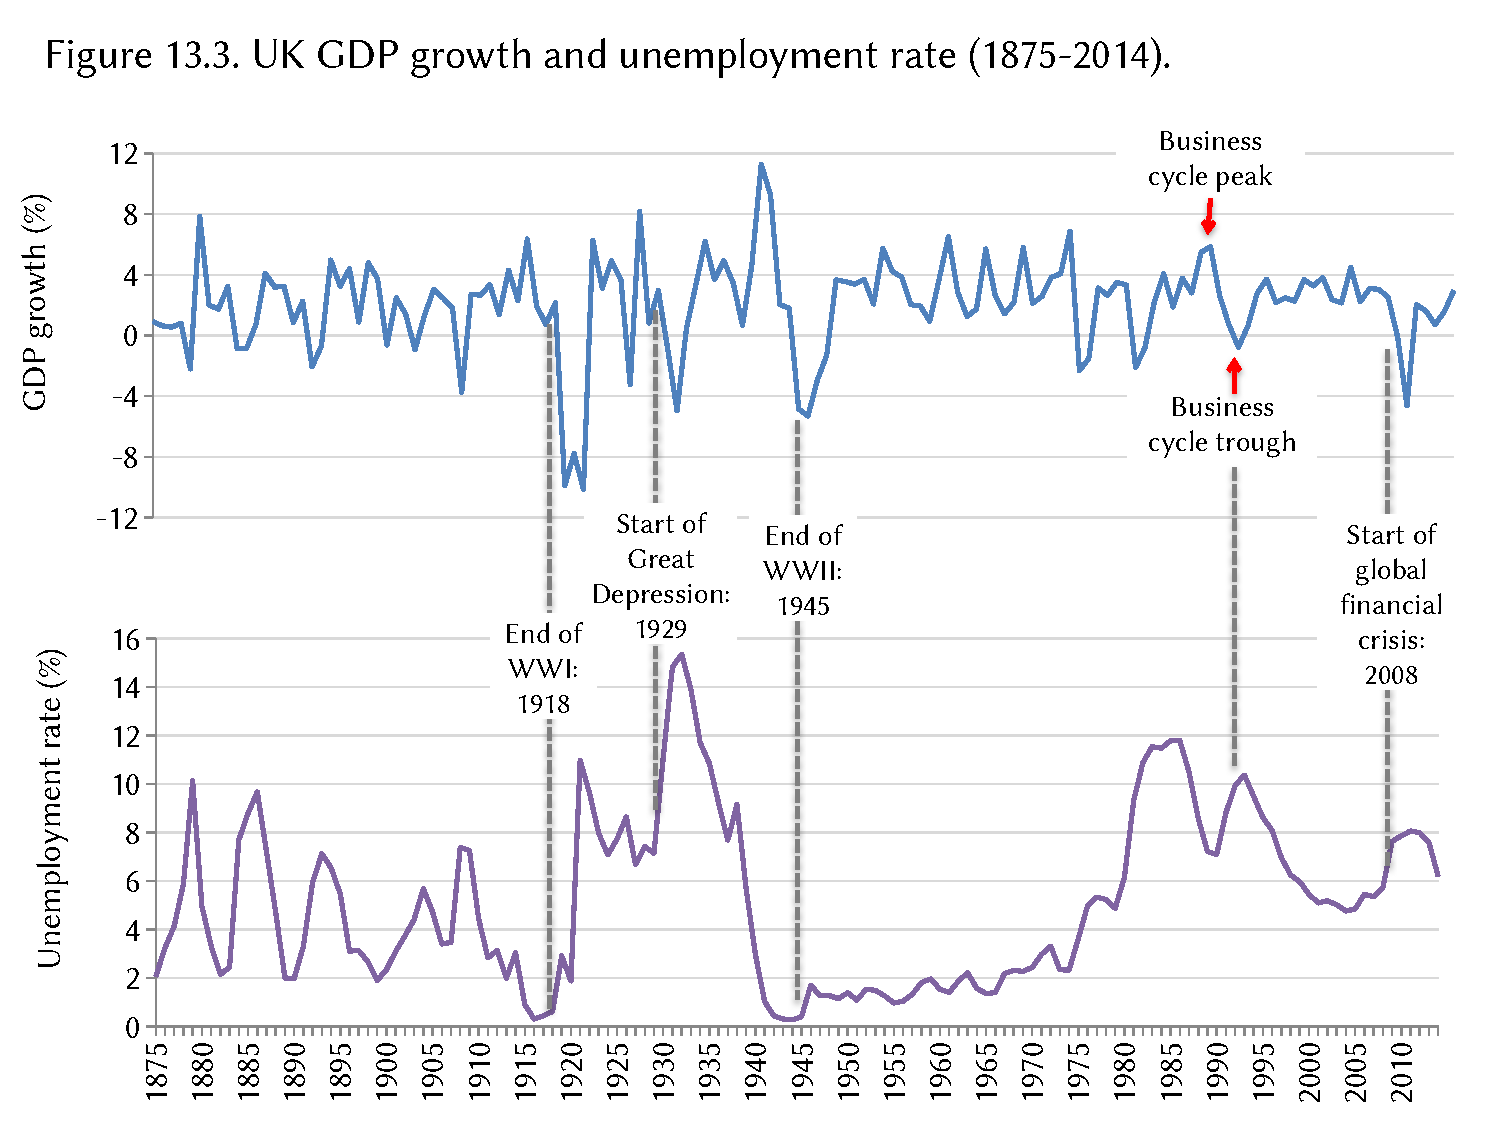
\includegraphics[width=\textwidth]{./figures/3.pdf}
        \end{figure}

    \end{column}
\end{columns}


\end{frame}

\begin{frame}{Okun's Law}
\label{slide:Okun_s_Law}
    \begin{columns}
        \begin{column}{0.3\textwidth}
            \begin{itemize}
                \item \textbf{Def:} a strong and stable \alert{negative} relationship between unemployment and GDP growth.
                \item Output falls → Unemployment rises → Well-being falls
            \end{itemize}
        \end{column}
        \begin{column}{0.7\textwidth}
            \begin{figure}
                \centering
                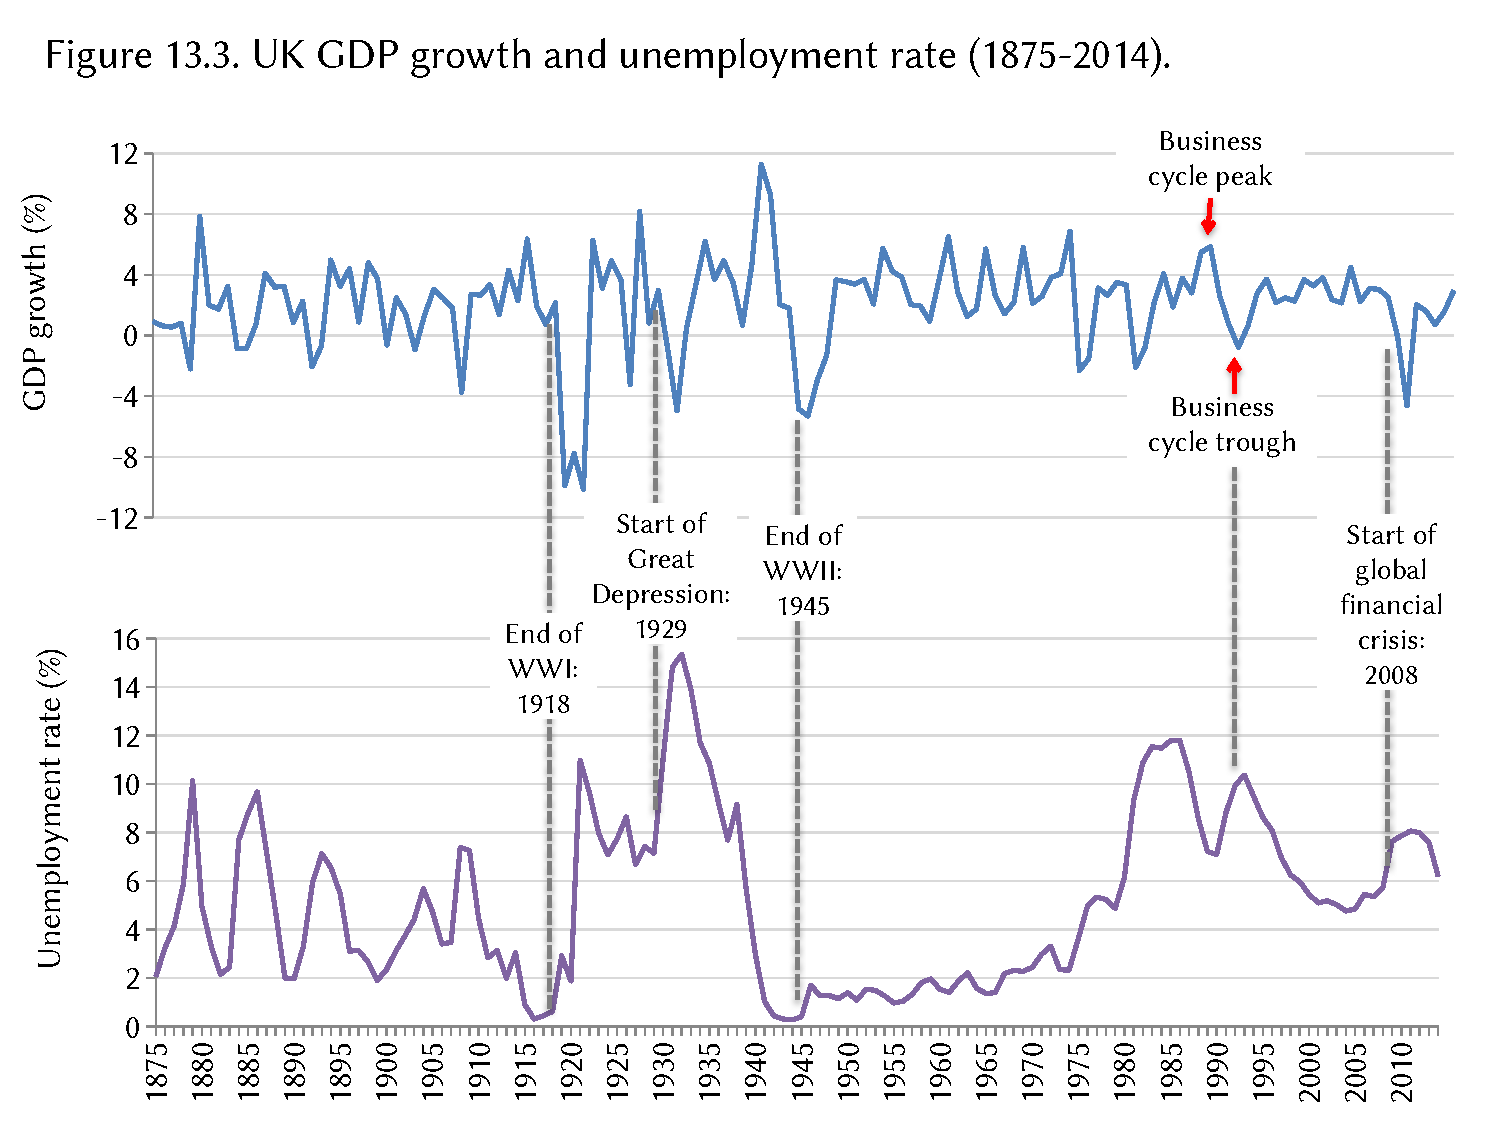
\includegraphics[width=\textwidth]{./figures/3.pdf}
            \end{figure}

        \end{column}
    \end{columns}

\end{frame}

\section[\faBalanceScale]{Measuring the Aggregate Economy}
\label{sec:Measuring_the_Aggregate_Economy}


\begin{frame}{Measurement of GDP}
\label{slide:Measurement_of_GDP}
    \begin{columns}
        \begin{column}{0.3\textwidth}
            $ 3 $ equivalent ways to measure GDP:
            \begin{enumerate}
                \item Total spending on domestic products
                \item Total domestic production (measured as value added)
                \item Total domestic income
            \end{enumerate}
        \end{column}
        \begin{column}{0.7\textwidth}
            \begin{figure}
                \centering
                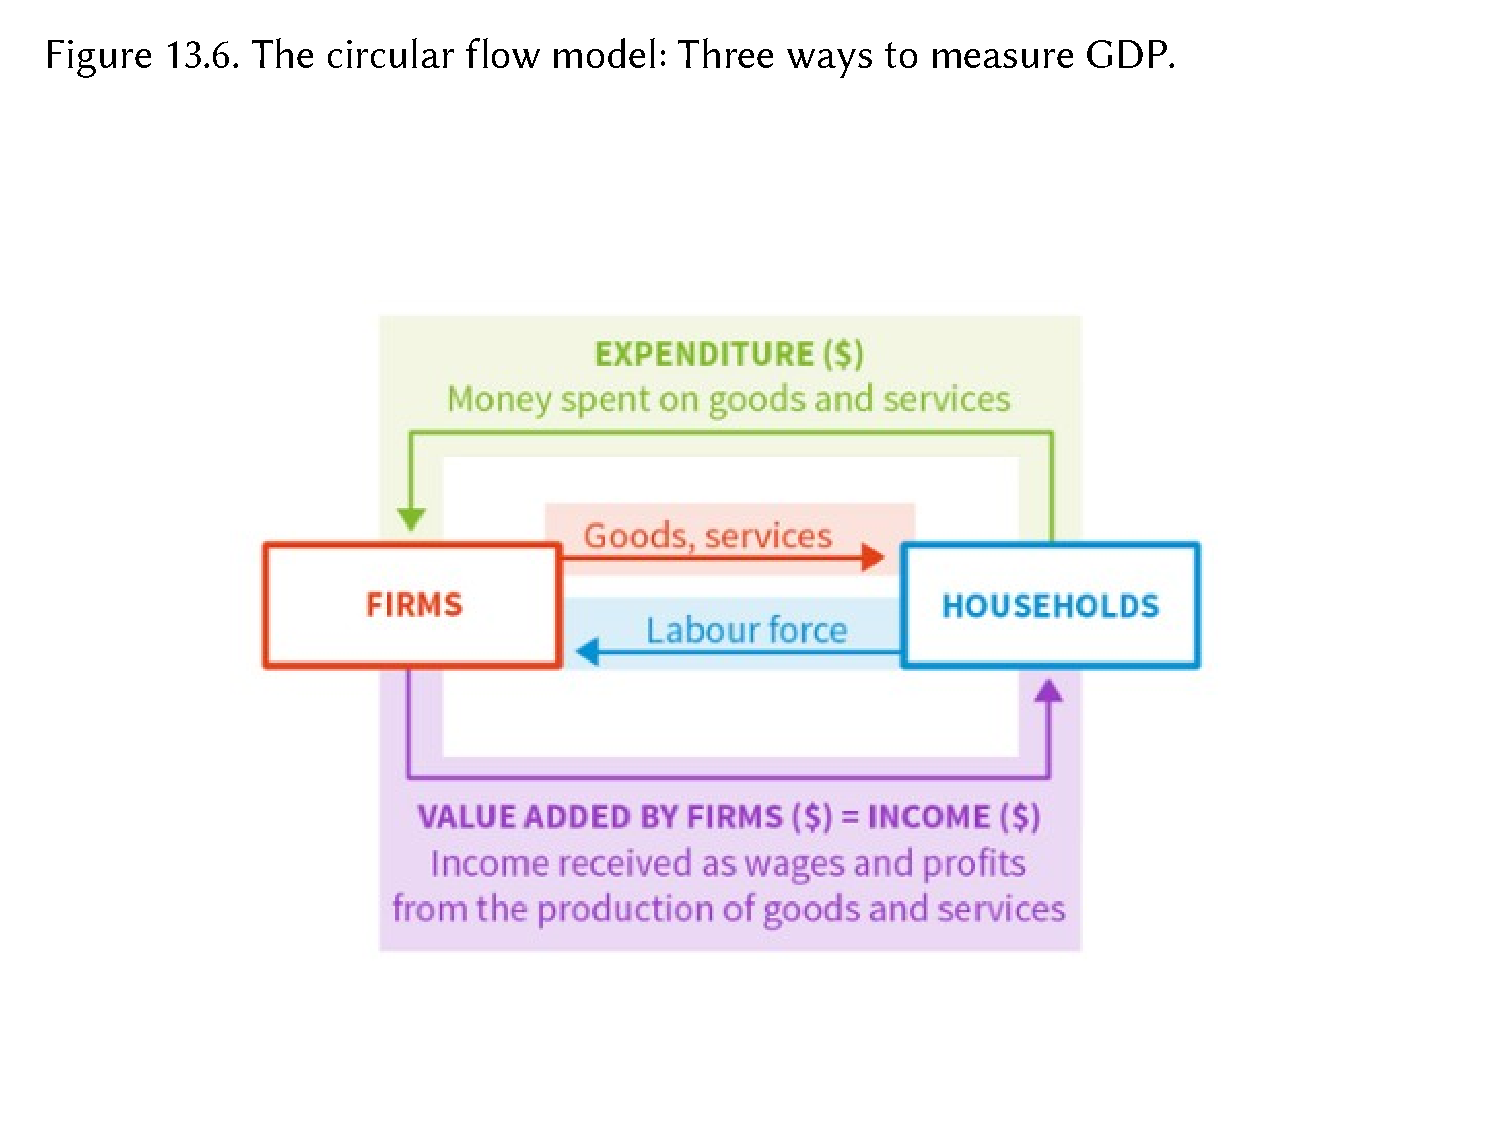
\includegraphics[width=\textwidth]{./figures/4.pdf}
            \end{figure}

        \end{column}
    \end{columns}

\end{frame}

\begin{frame}{Components of GDP}
\label{slide:Components_of_GDP}
    \begin{center}
        $ GDP = C + I + G + X - M $
    \end{center}
    \begin{itemize}
        \item Consumption ($ C $): Expenditure on consumer goods and services
        \item Investment ($ I $): Expenditure on newly produced capital goods (incl. equipment, buildings, and inventories: unsold output)
        \item Government spending ($ G $): Government expenditure on goods and services (excluding transfers to avoid double-counting)
        \item Net exports (trade balance): Exports ($ X $) minus imports ($ M $)
    \end{itemize}

\end{frame}

\begin{frame}{Components of GDP (Cont.)}
\label{slide:Components_of_GDP__Cont__}
    \begin{figure}
        \centering
        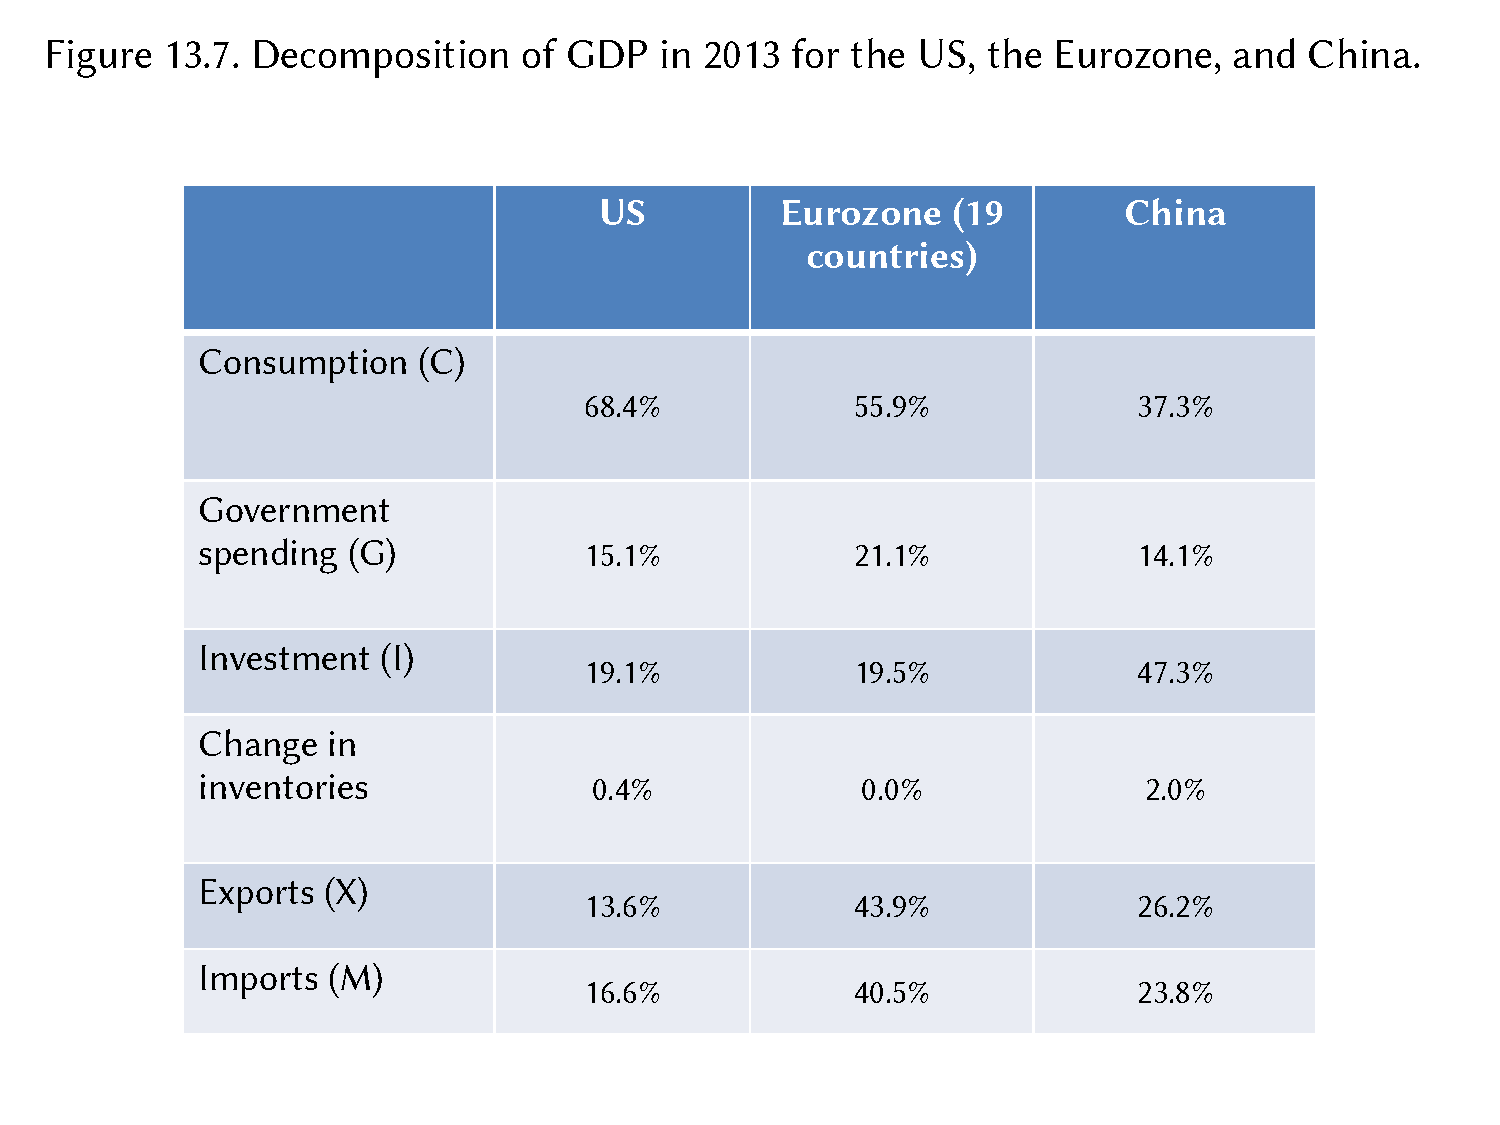
\includegraphics[width=.8\textwidth]{./figures/5.pdf}
        \caption{Private Consumption ($C$) makes the largest share \ldots $ C $ is the most important?}
    \end{figure}
\end{frame}

\begin{frame}{Components of GDP growth}
\label{slide:Components_of_GDP_growth}
    \begin{figure}
        \centering
        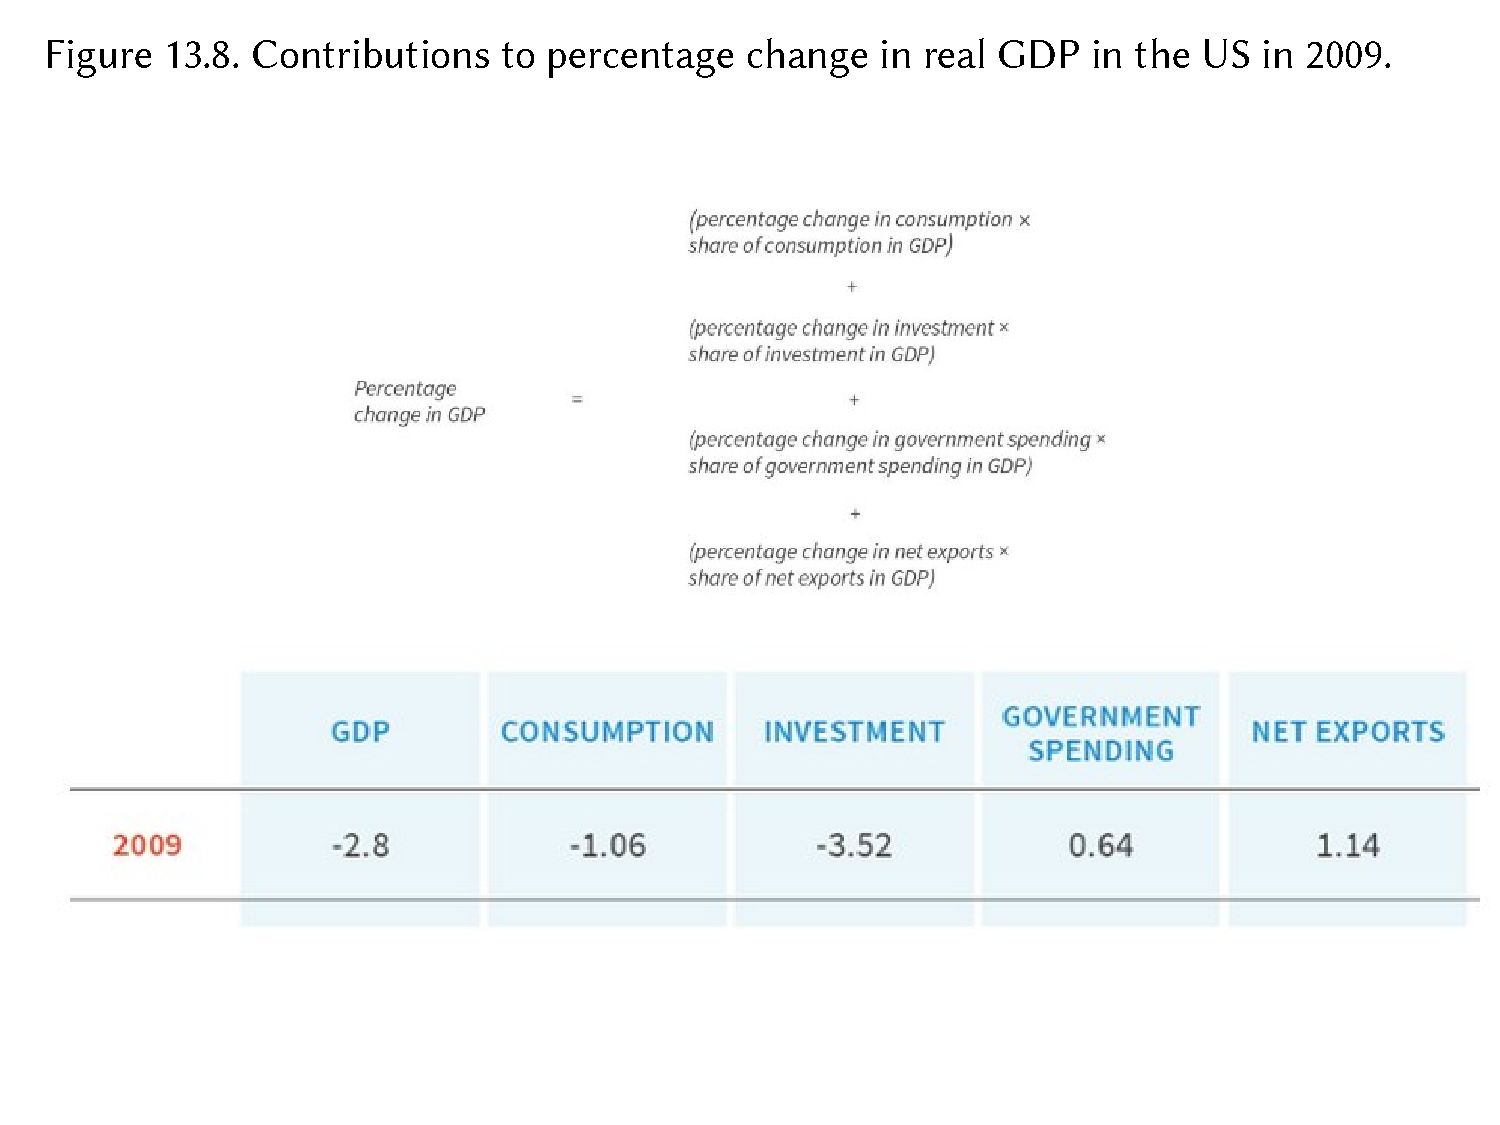
\includegraphics[width=.8\textwidth]{./figures/6.pdf}
        \caption{In terms of \alert{percentage change}, investment is the most volatile!}
    \end{figure}
\end{frame}

\section[\faLineChart]{Economics Fluctuation}
\label{sec:Economics_Fluctuation}

\begin{frame}{Shocks}
\label{slide:Shocks}
    \begin{center}
        \textbf{Def:} an \alert{unexpected} event to agent(s)
    \end{center}
    There are two broad types of shocks:
    \begin{enumerate}
        \item \textbf{idiosyncratic shocks}: Good or bad fortune strikes the household
        \begin{itemize}
            \item Self-insurance: saving and borrowing; other HH are not involved.
            \item Co-insurance: support from social network or government.
        \end{itemize}
        \item \textbf{aggregate shocks}: Good or bad fortune strikes the entire economy
        \begin{itemize}
            \item Co-insurance is less effective \alert{but even more necessary}
            \item In farming economies of the past that were based in \alert{volatile climates}, people practised co-insurance based on \alert{trust, reciprocity, and altruism}.
        \end{itemize}

    \end{enumerate}


\end{frame}

\begin{frame}{Consumption Smoothing}
\label{slide:Consumption_Smoothing}
    \begin{columns}
        \begin{column}{0.3\textwidth}
            \begin{itemize}
                \item<only@1> Households make lifetime consumption plans based on expectations about the future, and react to shocks:
                \item<only@2> \red{Red line}: long-run consumption if shocks are permanent
                \item<only@2> \blue{Blue line}: Income flow at each period (Income shocks)
                \item <only@3> Consumption smoothing: do not change long-run consumption if shocks are \alert{temporary}
            \end{itemize}
        \end{column}
        \begin{column}{0.7\textwidth}
            \begin{figure}
                \centering
                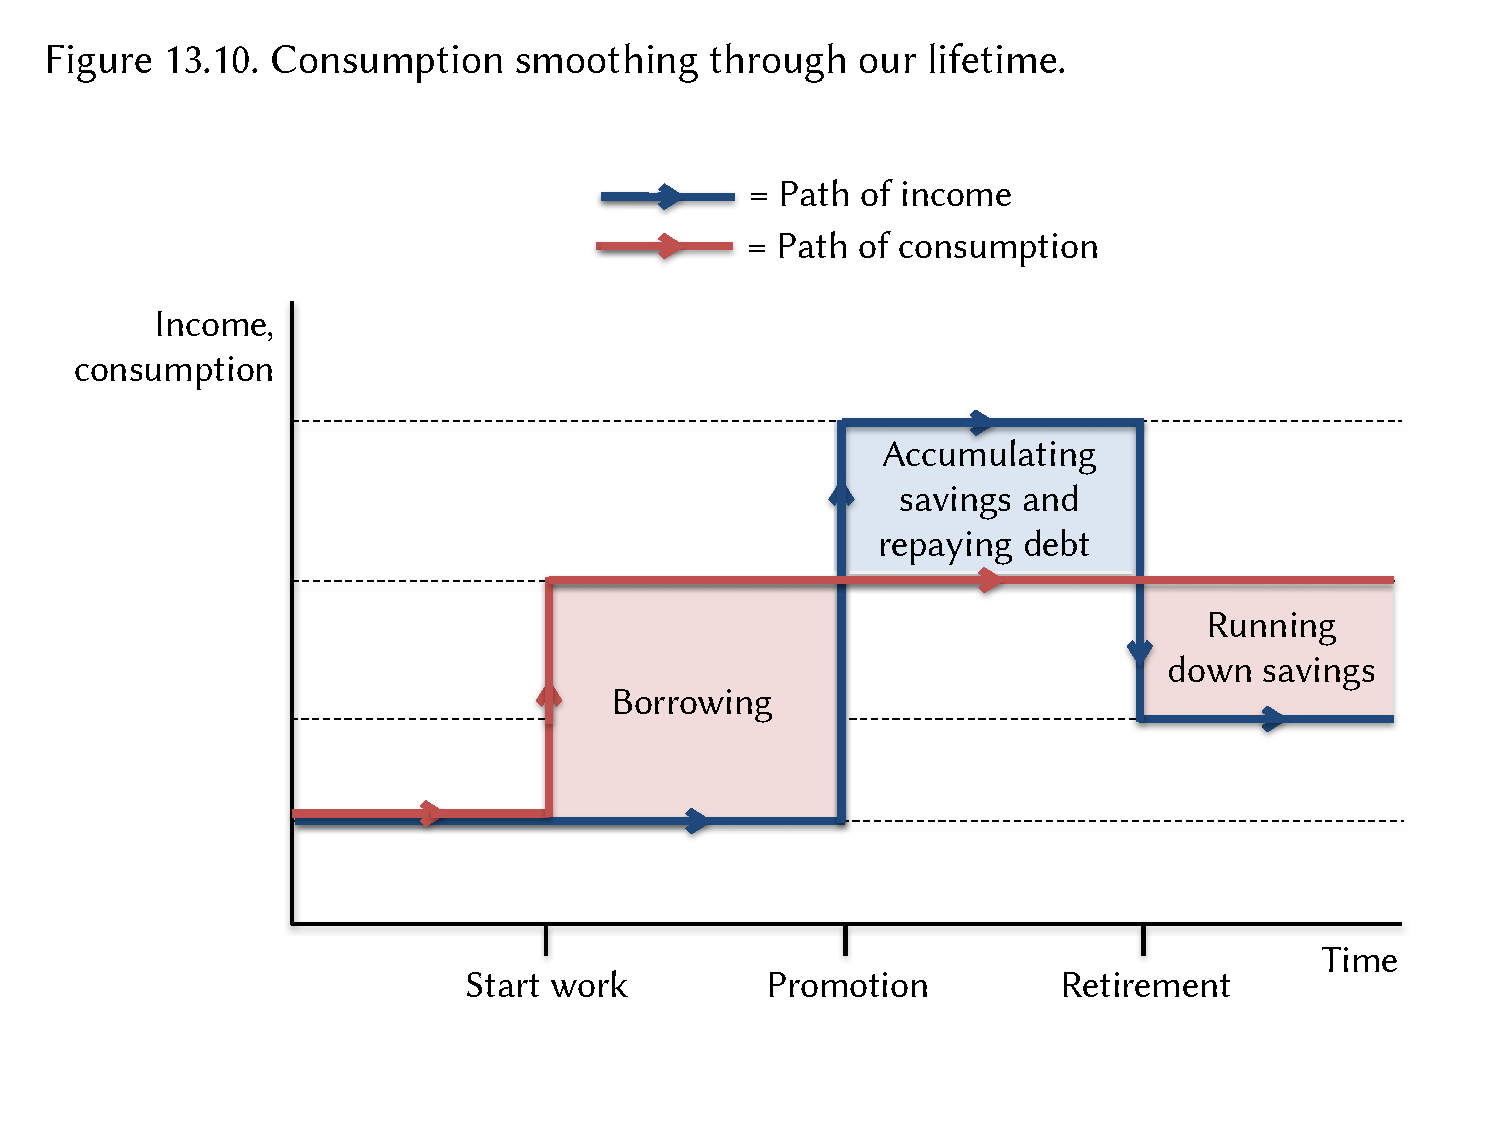
\includegraphics[width=\textwidth]{./figures/7.pdf}
            \end{figure}

        \end{column}
    \end{columns}

\end{frame}

\begin{frame}{Limitation on Consumption Smoothing}
\label{slide:Limitaion_on_Consumption_Smoothing}
    \begin{columns}
        \begin{column}{0.3\textwidth}
            \begin{itemize}
                \item <only@1>\textbf{Credit constraints}: limits on amount borrowed/ability to borrow.
                \item <only@1>The households unable to adjust to a temporary income shock have lower welfare.
                \item <only@2>Another angle using $ C-C' $ figure
                \item <only@2> $ A' $: credit-constrained allocation
                \item <only@2> $ A'' $: credit-unconstrained allocation
                \item <only@3> \textbf{Weakness of will}: inability to commit to beneficial future plans.
                \item <only@3> A household is able to smooth consumption but doesn't, and may regret it later.
            \end{itemize}
        \end{column}
        \begin{column}{0.7\textwidth}
            \only<1>{
            \begin{figure}
                \centering
                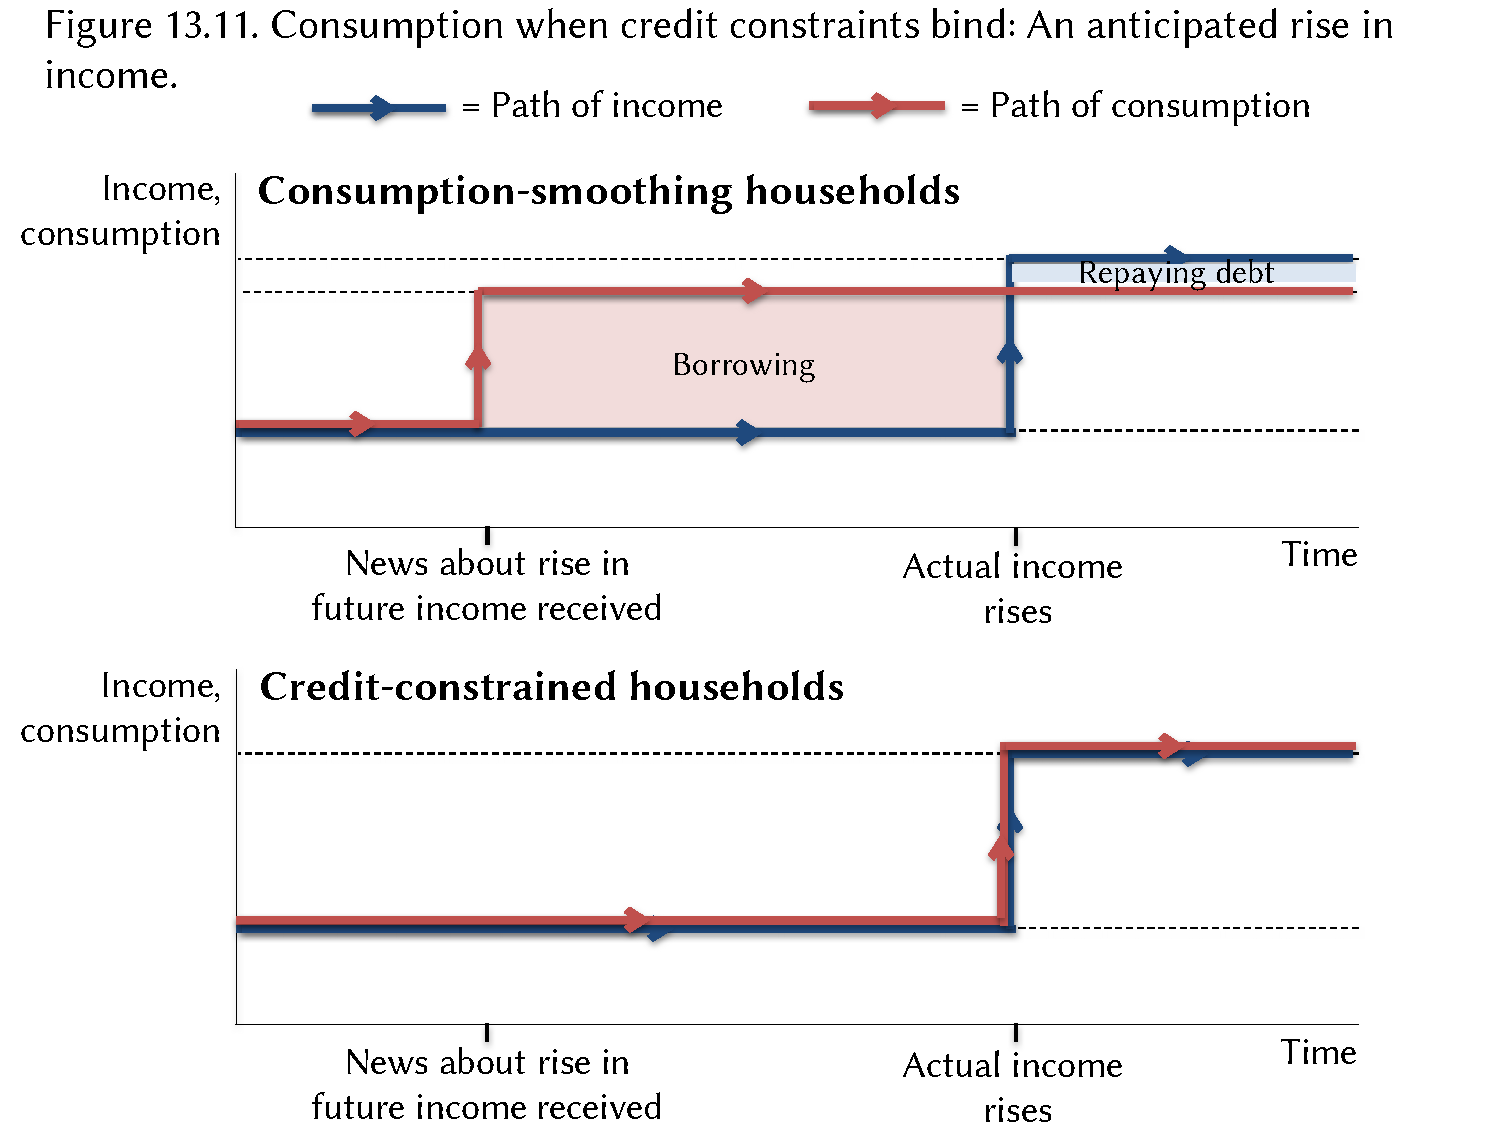
\includegraphics[width=\textwidth]{./figures/8.pdf}
            \end{figure}
            }
            \only<2>{
            \begin{figure}
                \centering
                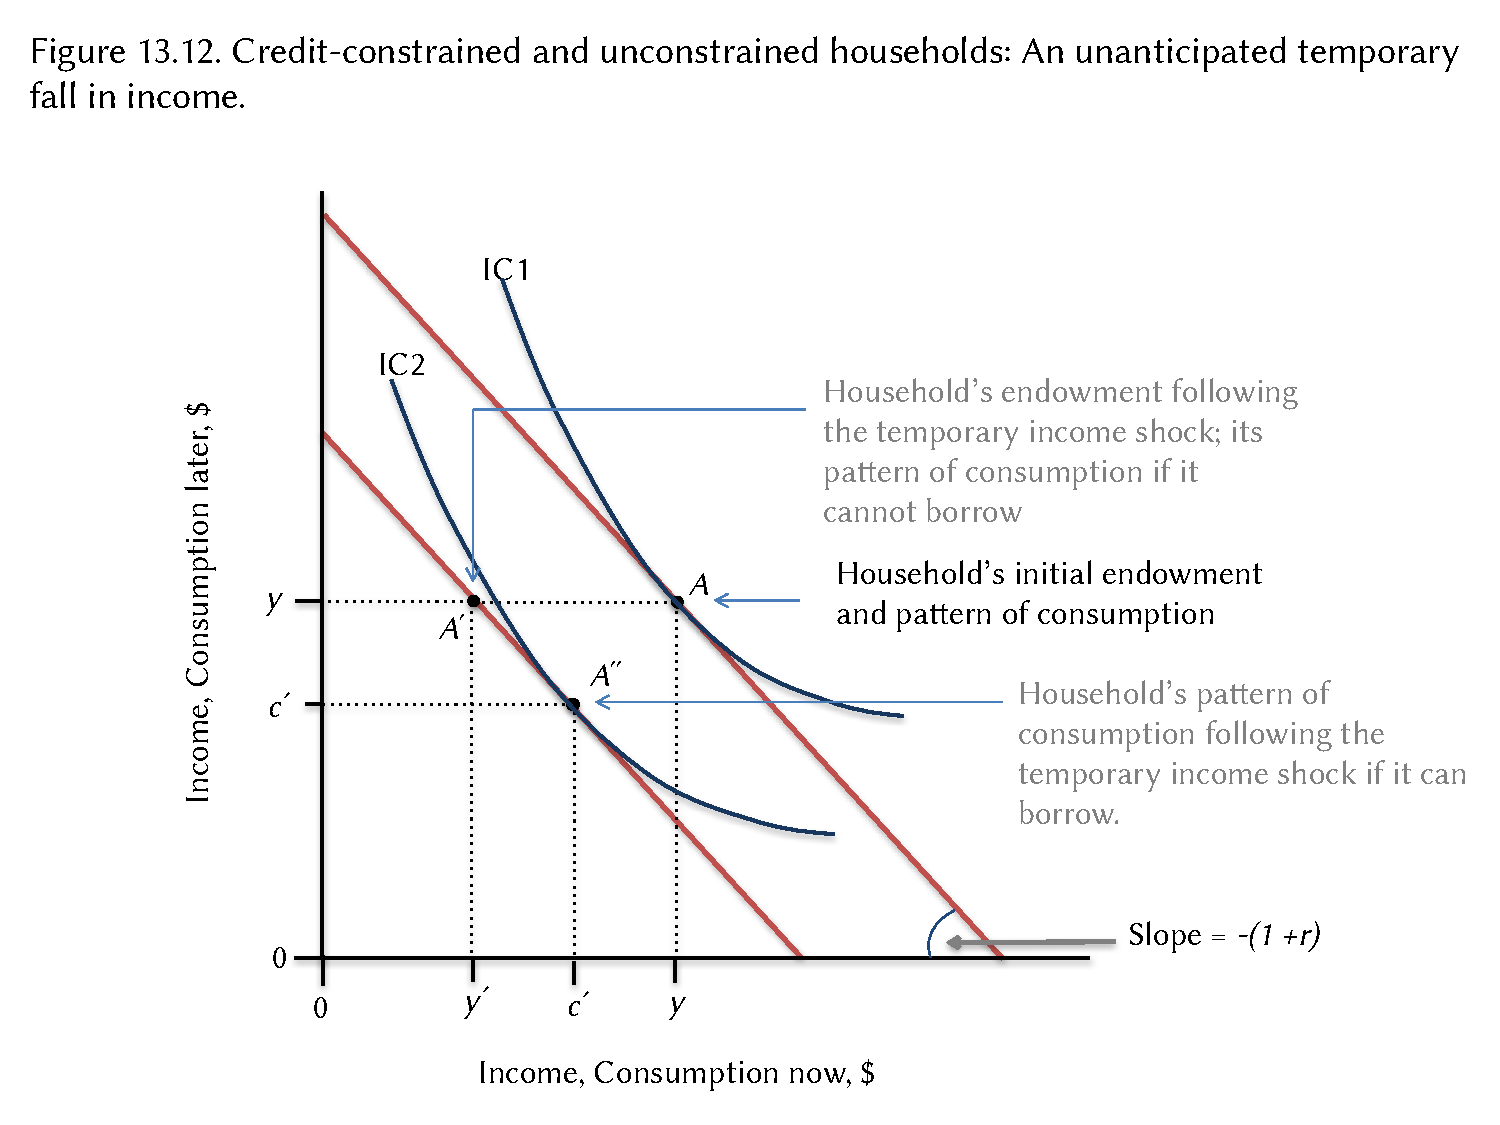
\includegraphics[width=\textwidth]{./figures/9.pdf}
            \end{figure}
            }
            \only<3>{
            \begin{figure}
                \centering
                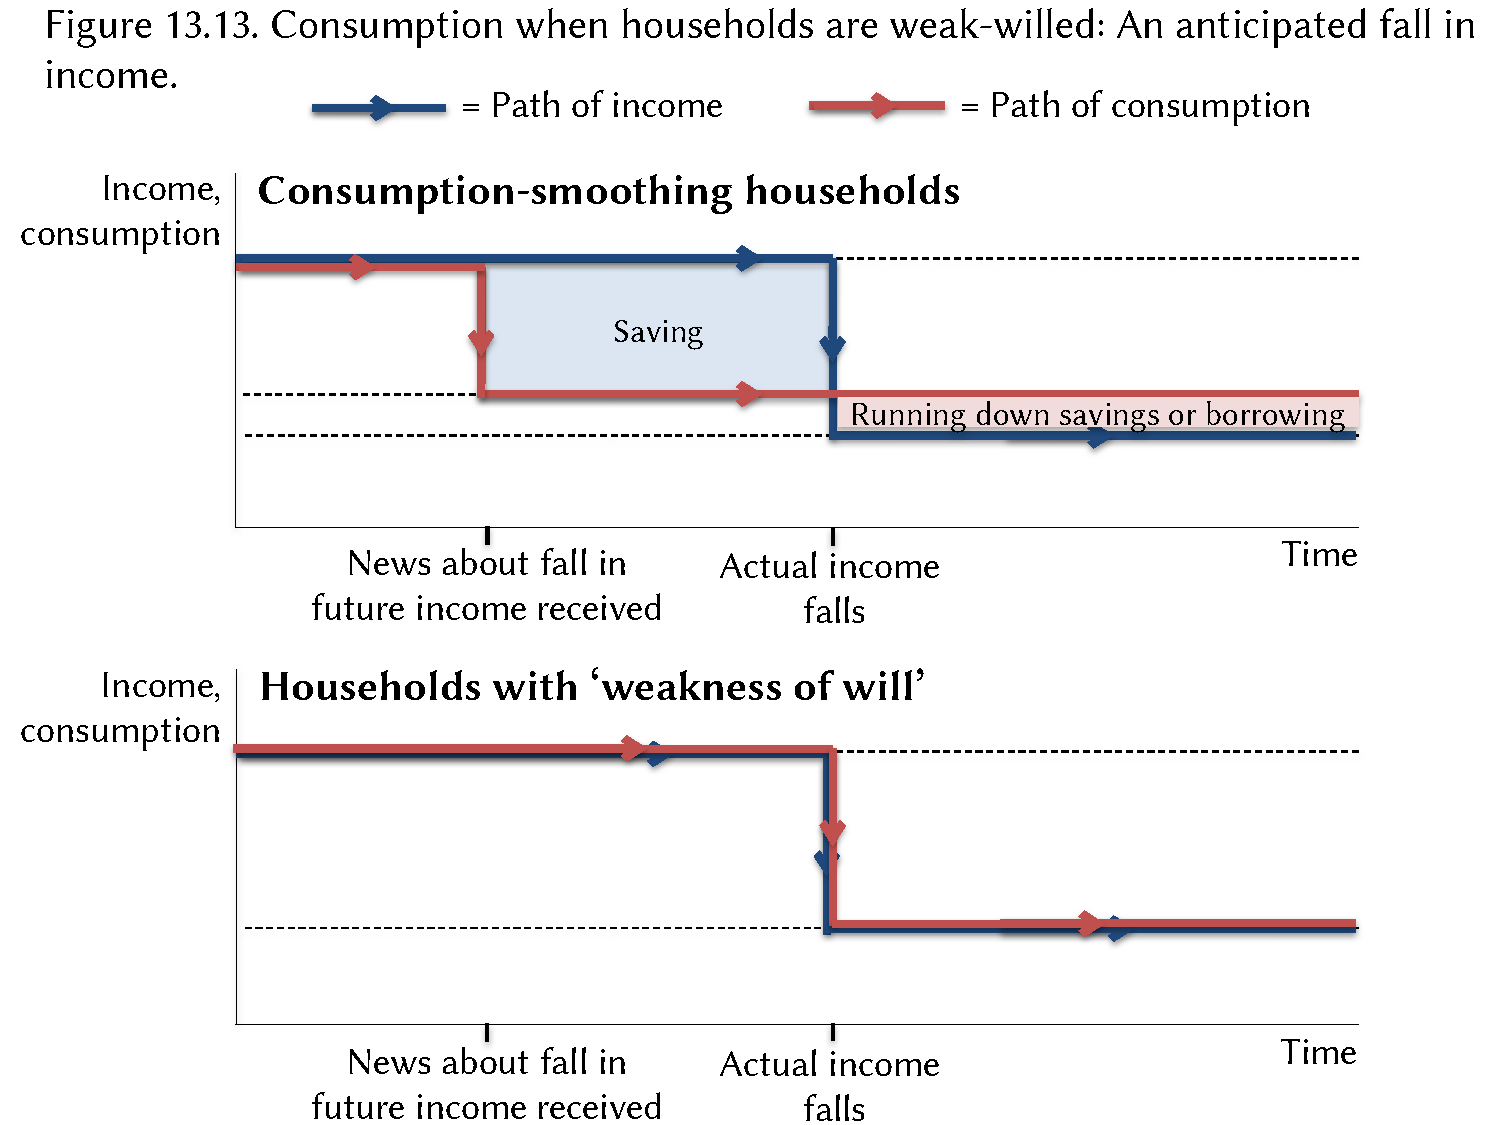
\includegraphics[width=\textwidth]{./figures/10.pdf}
            \end{figure}

            }
        \end{column}
    \end{columns}

\end{frame}

\begin{frame}{Optimal Investment}
\label{slide:Optimal_Investment}
    \begin{center}
        \textit{Why investment is volatile}?
    \end{center}
    \begin{itemize}
        \item Firms don't ``smooth'' investment; investment is \alert{lumpy}.
        \begin{itemize}
            \item Firms' goal is to max profit, and disband a firm is common
        \end{itemize}
        \item High demand → high capacity utilisation → investment → even higher demand
        \item Investment decisions depend on firms' expectations about future demand
    \end{itemize}
\end{frame}

\begin{frame}{Investment as a coordination game}
\label{slide:Investment_as_a_coordination_game}
    \begin{figure}
        \centering
        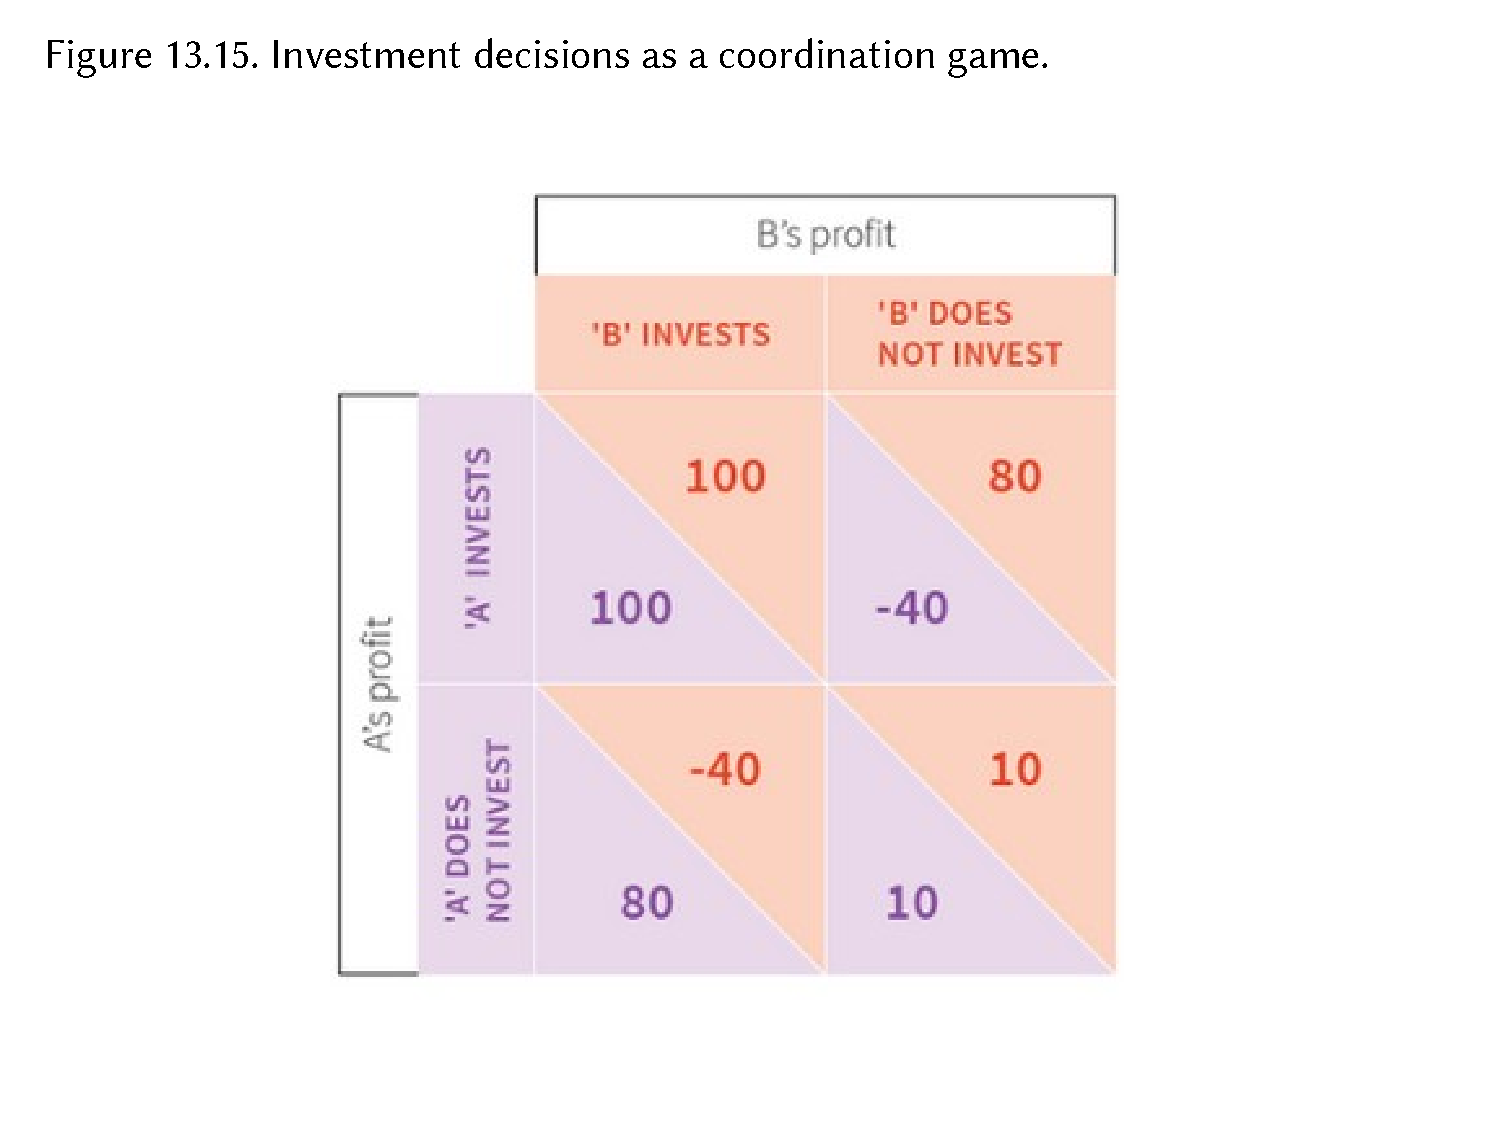
\includegraphics[width=\textwidth]{./figures/11.pdf}
    \end{figure}
\end{frame}

\begin{frame}{Confidence Matters}
\label{slide:Confidence_Matters}
    \begin{itemize}
        \item \textbf{Business confidence} coordinates firms to invest at the same time.
        \item The benefits of \alert{coordinating investment} makes cycles \textbf{self-reinforcing}.
        \item Firms respond positively to the growth of demand in the economy $ \Rightarrow  $ why investment is more volatile than GDP.
    \end{itemize}


\end{frame}

\begin{frame}{Other Components}
\label{slide:Other_Components}
    \begin{itemize}
        \item Government spending is \alert{less volatile} than investment (does not depend on business confidence)
        \item Exports depend on \alert{demand from other countries}, so will fluctuate according to the business cycles of major export markets.
    \end{itemize}
\end{frame}

\section[\faMoney]{Inflation}
\label{sec:Inflation}


\begin{frame}{Inflation, GDP and Unemployment}
\label{slide:Inflation__GDP_and_Unemployment}
    \begin{center}
        Inflation: an increase in the \alert{general price level} in the economy

        Inflation tends to be lower during recessions (high unemployment)
    \end{center}
    \begin{figure}
        \centering
        \only<1>{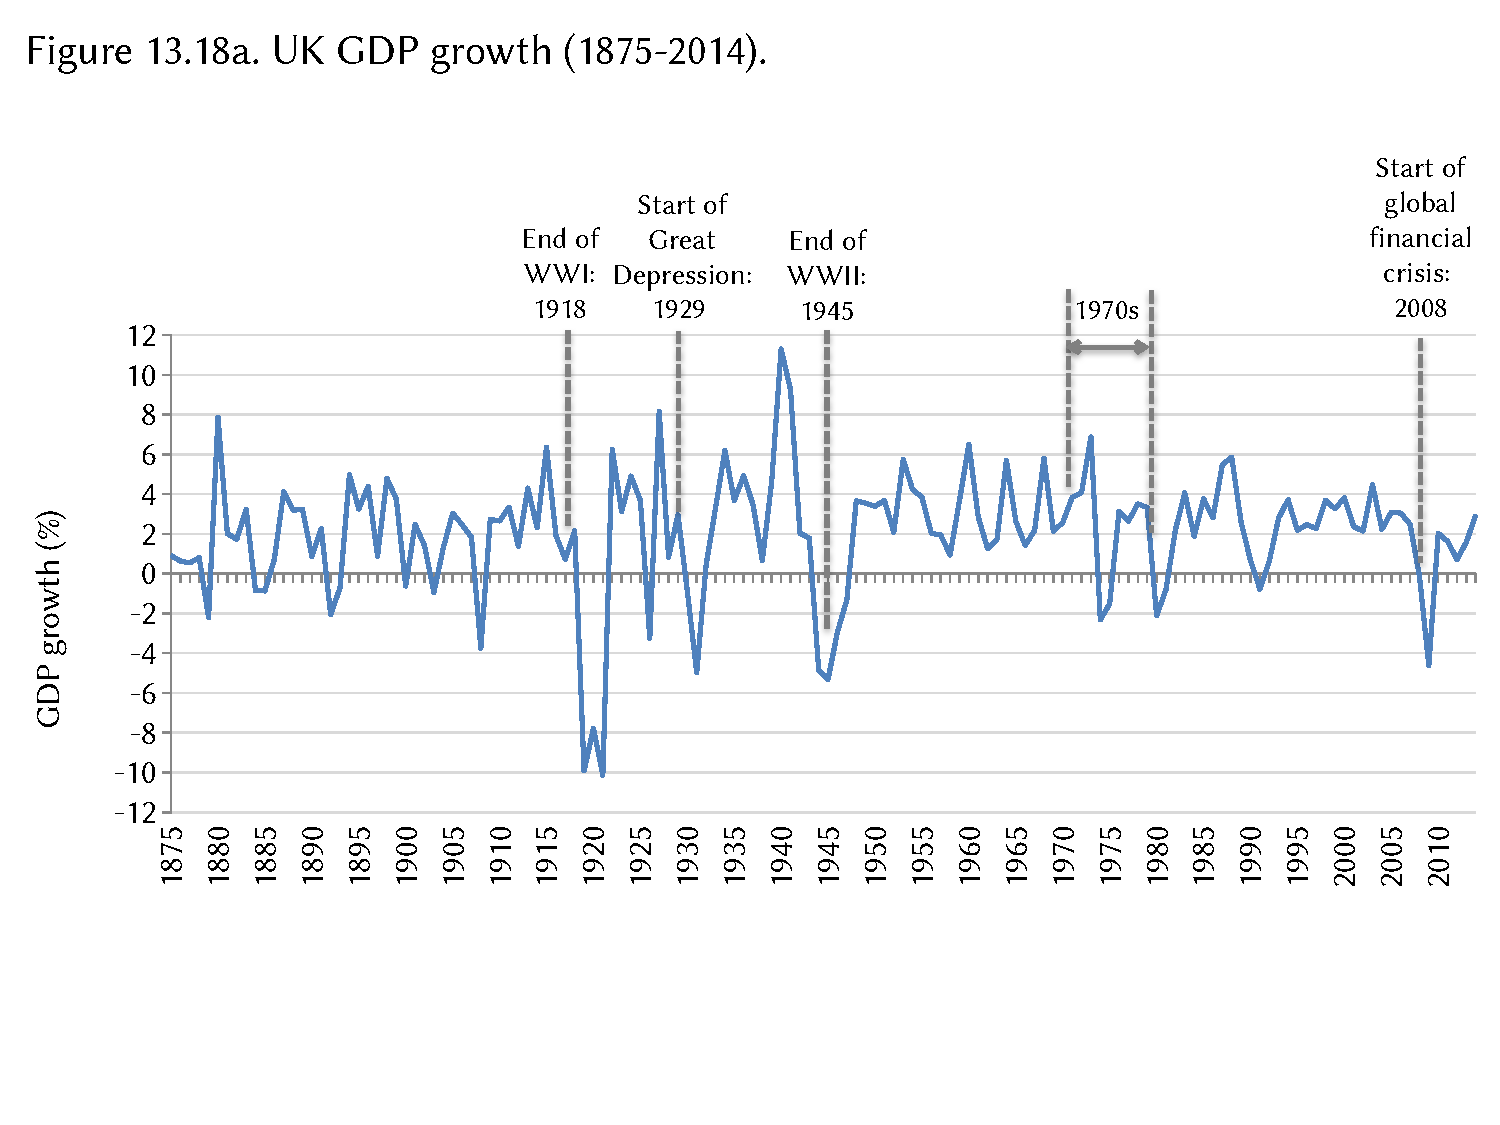
\includegraphics[width=.9\textwidth]{./figures/12.pdf}}
        \only<2>{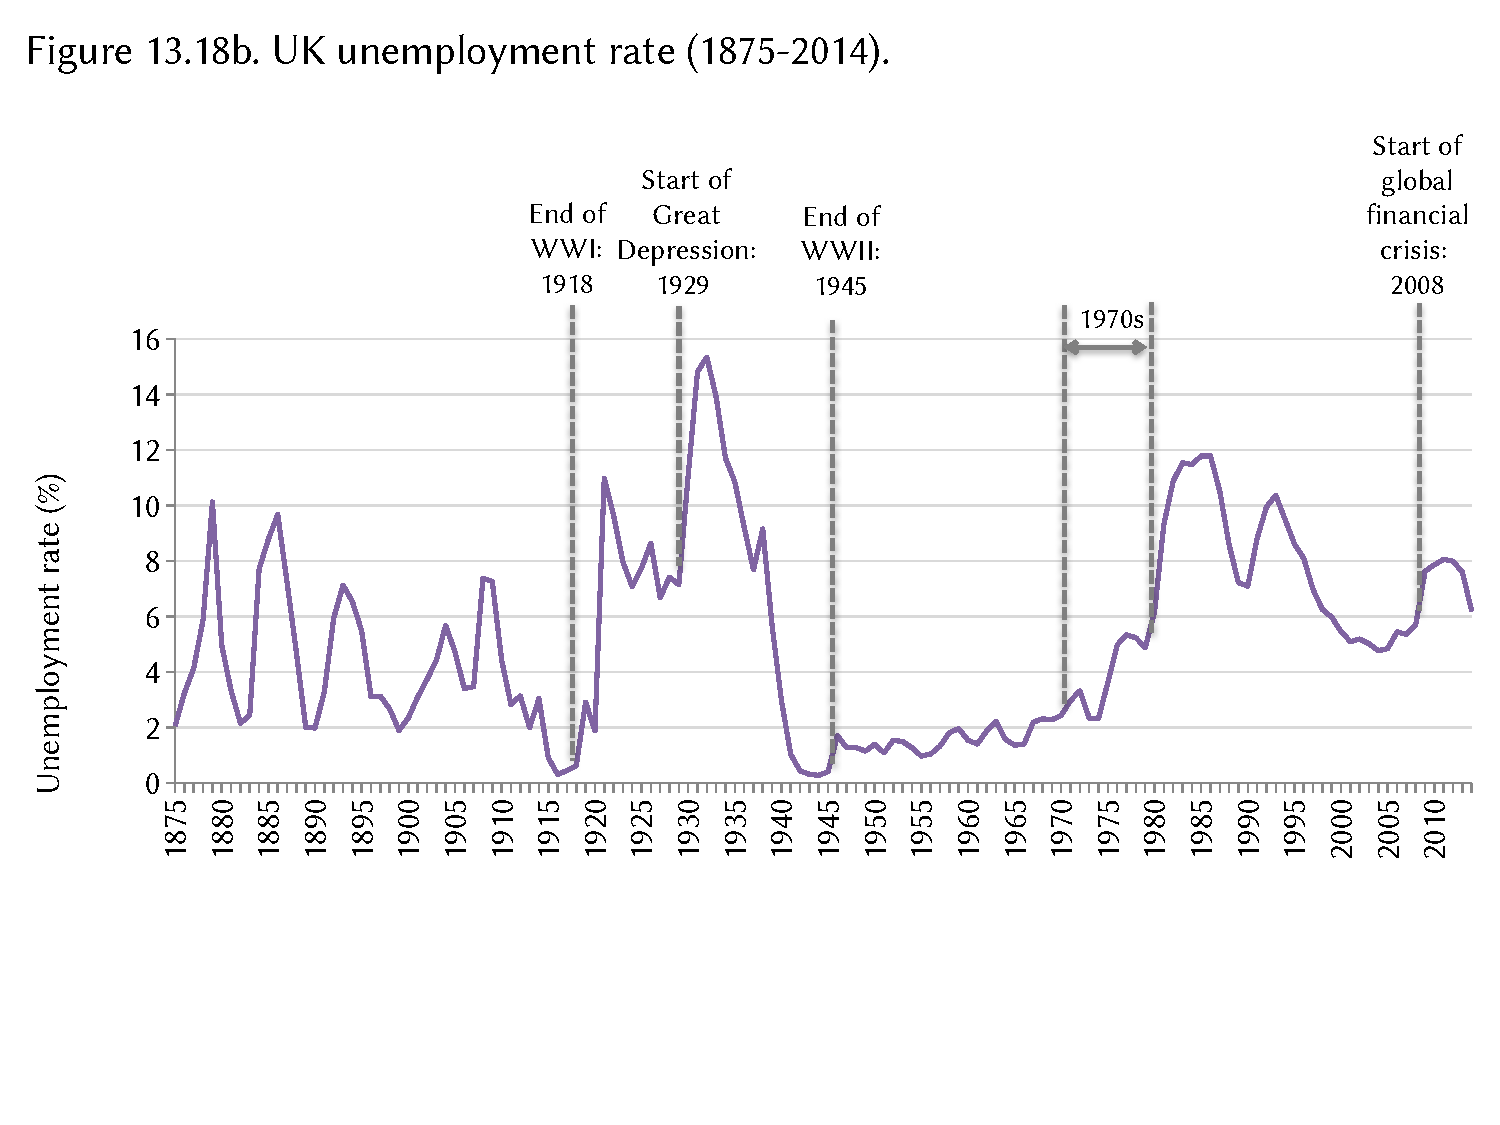
\includegraphics[width=.9\textwidth]{./figures/13.pdf}}
        \only<3>{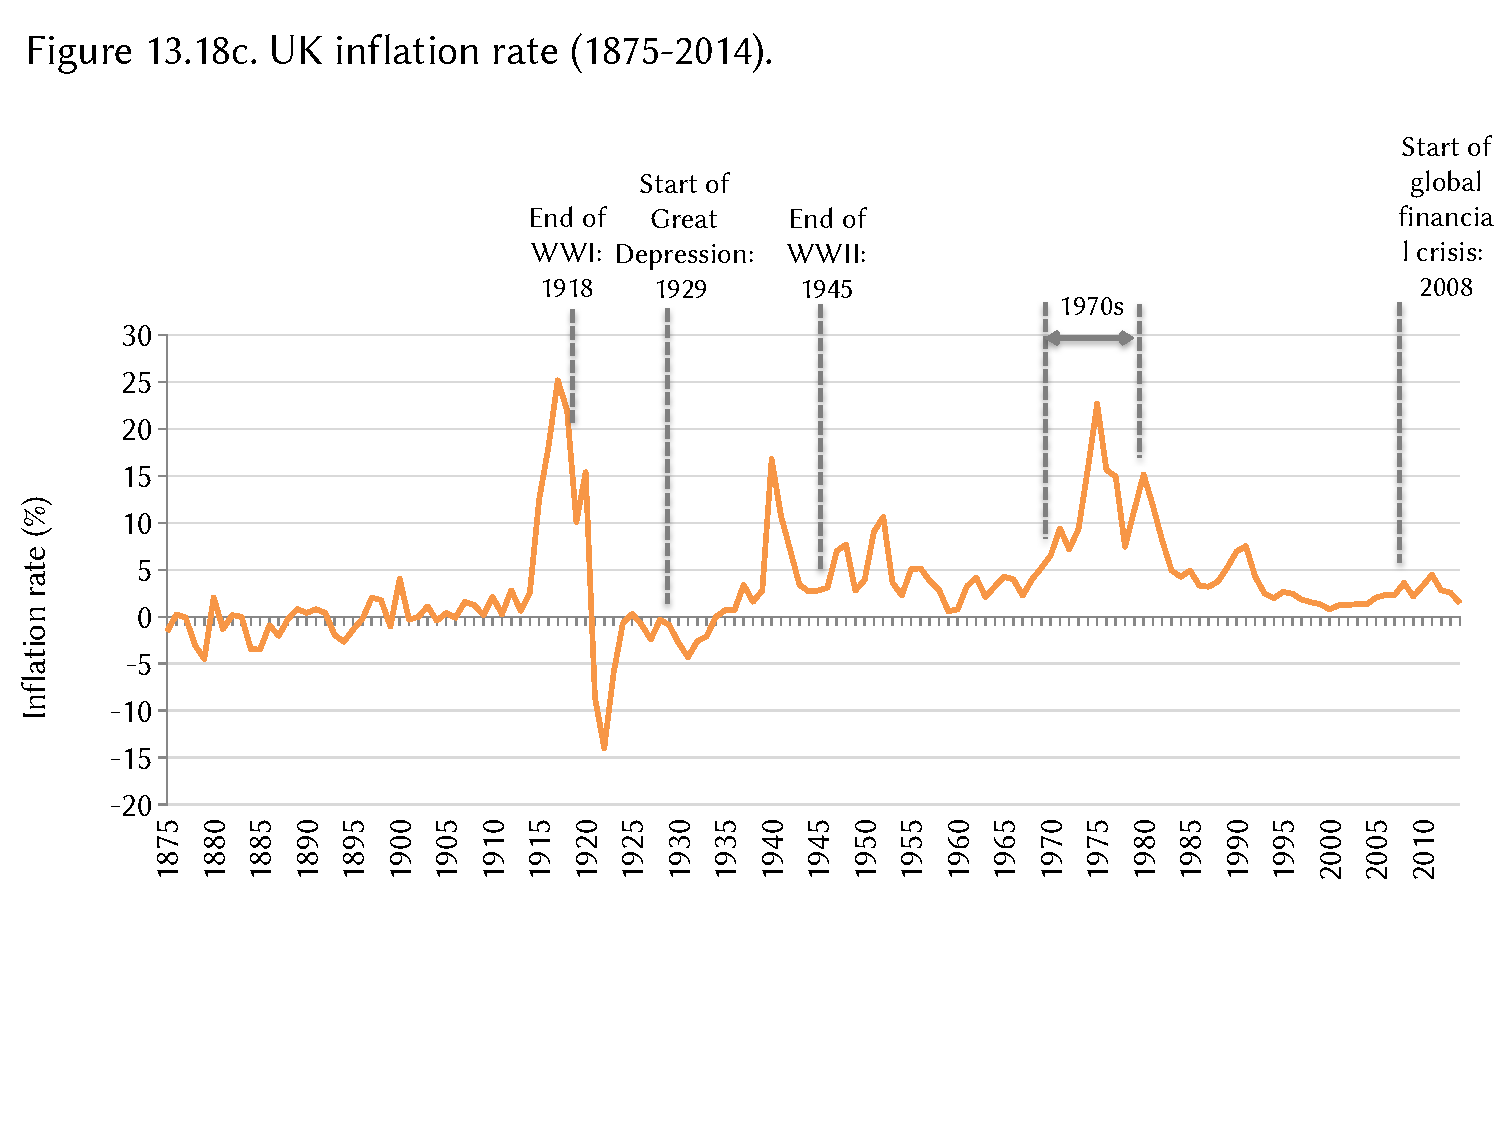
\includegraphics[width=.9\textwidth]{./figures/14.pdf}}
    \end{figure}

\end{frame}

\begin{frame}{Cross Country Trend in Inflation}
\label{slide:Cross_Country_Trend_in_Inflation}
    \begin{itemize}
        \item<only@1> Upward spikes in inflation during economic crises
        \item<only@2> general downward trend since 1970s
        \item<only@3> inflation tends to be higher in poor than in rich countries
    \end{itemize}
    \begin{figure}
        \centering
        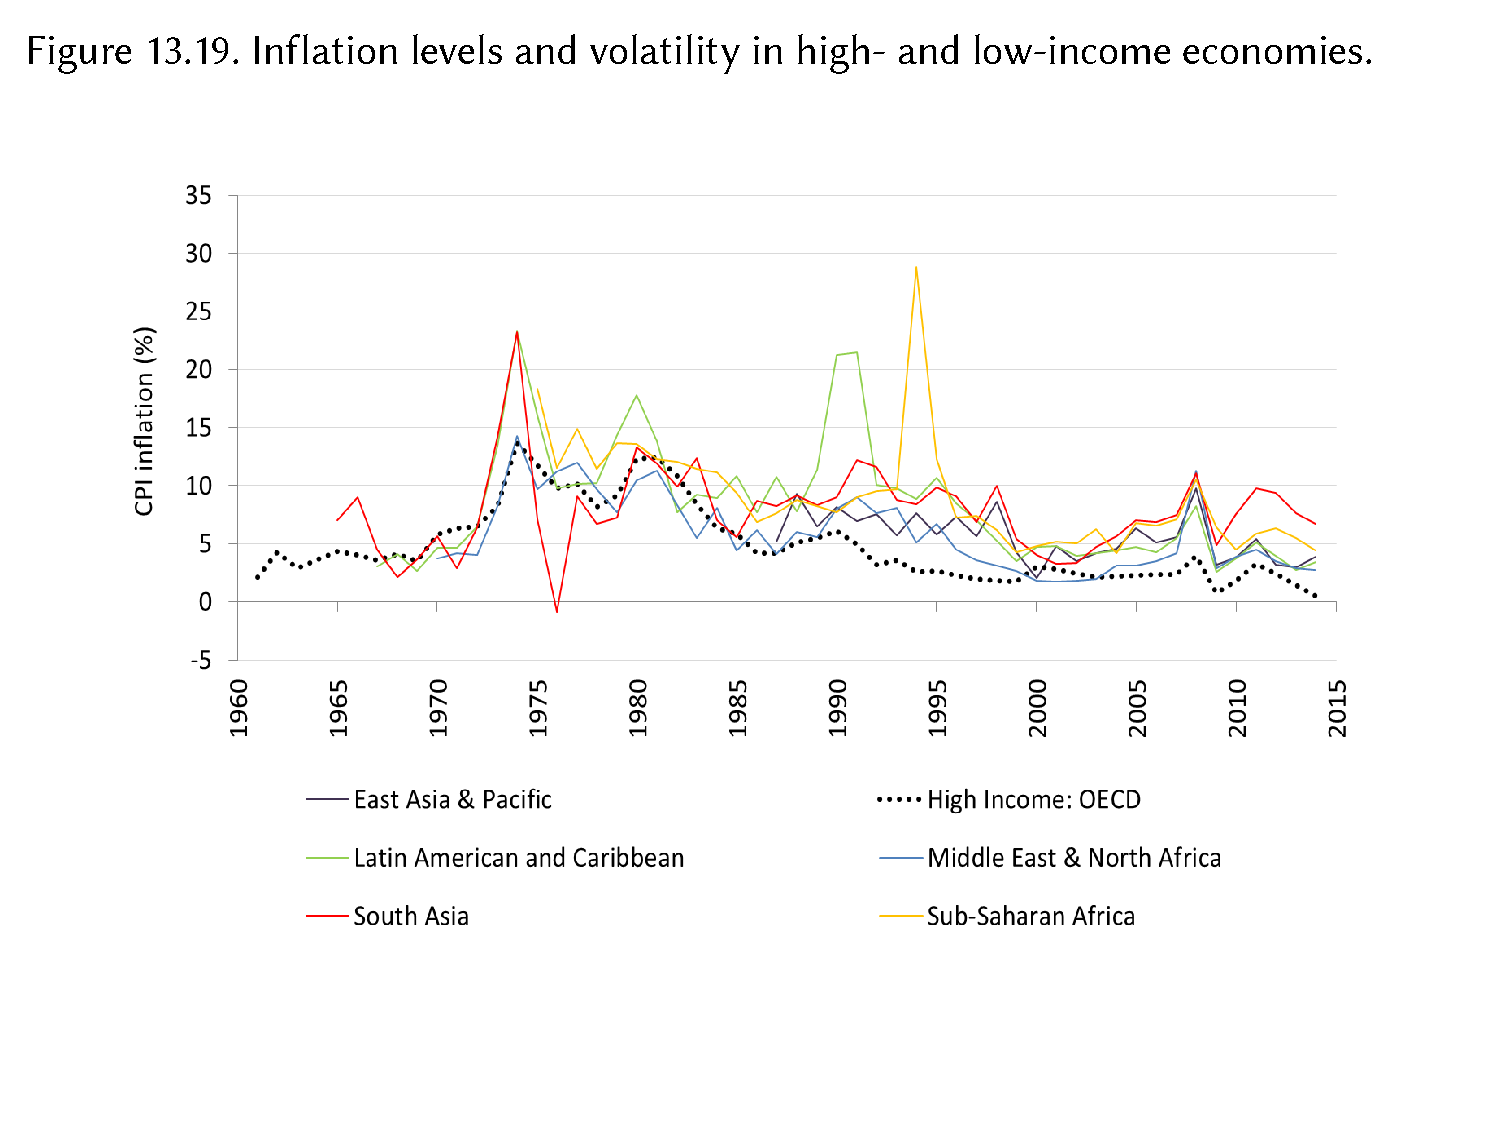
\includegraphics[width=.9\textwidth]{./figures/15.pdf}
    \end{figure}

\end{frame}

\begin{frame}{Measuring inflation}
\label{slide:Measuring_inflation}
    \begin{enumerate}
        \item \textbf{Consumer Price Index (CPI)}: general level of prices that consumers have to pay for goods and services, including consumption taxes
        \begin{itemize}
            \item measure the ``cost of living''
            \item Based on \alert{consumption basket}, different across countries
            \item Common measure of inflation $ = $ change in CPI
        \end{itemize}
        \item \textbf{GDP deflator}: measure of the level of prices for domestically produced output (ratio of nominal to real GDP)
        \begin{itemize}
            \item Tracks prices of components of GDP $(C, I, G, NX)$
            \item Allows GDP to be compared across countries and over time
        \end{itemize}

    \end{enumerate}


\end{frame}


%\section{Appendix}
%\label{sec:Appendix}

%\appendix
%% -------------------------------------------
%\setbeamertemplate{headline}
%{
%\setbeamercolor{section in head/foot}{fg=black, bg=white}
%\vskip1em \tiny \insertsectionnavigationhorizontal{1\paperwidth}{\hspace{0.50\paperwidth}}{}
%}
%%------------------------------------------
%% \begin{frame}\frametitle{}
%% \begin{columns}
%% \label{Appendix}
%% \column{1\linewidth}
%% \centering
%% {\Large \alert{Appendix}}
%% \end{columns}
%% \end{frame}
%%------------------------------------------
%\begin{frame}[allowframebreaks]{References}
%\footnotesize
%\bibliographystyle{$BIB_STYLE}
%\bibliography{$BIBFILE}
%\end{frame}

\end{document}
